\documentclass[a4paper,11pt]{report}

\usepackage[T1]{fontenc}
\usepackage[utf8]{inputenc}
\usepackage[italian]{babel}

\usepackage{chemmacros}
\usepackage{mathtools}
\usepackage{graphicx}
\usepackage{amsfonts}
\usepackage{amsthm}
\usepackage{amsmath}
\usepackage{amssymb}
\usepackage{fancyhdr}
\usepackage{float}
\usepackage{geometry}
\geometry{a4paper, top=2.5cm, bottom=2cm, left=2cm, right=2cm}
\usepackage{hyperref}
\hypersetup{
	colorlinks=true,
	linkcolor=black,
	filecolor=blue,
	citecolor = black,      
	urlcolor=cyan,
}

\newtheorem*{es}{Esempio}

\begin{document}
	\date{}
	\author{Marco Militello}
	\title{Chimica}
	\maketitle
	\tableofcontents
	\newpage
	
\chapter{Introduzione}
La chimica è lo studio della materia, delle sue proprietà, delle trasformazioni subite dalla materia e dell'energia associata a queste trasformazioni
\begin{description}
	\item[Materia] Tutto ciò che ha una massa e un volume
	\item[Composizione] I tipi e le quantità di sostanze più semplici che costituiscono la materia
	\item[Proprietà] Le caratteristiche che conferiscono a ciascuna sostanza la sua identità esclusiva 
\end{description}
\section{Stati aggregazione della materia}
\begin{itemize}
	\item Un \emph{solido} ha forma e volumi fissi. I solidi possono essere duri, teneri, rigidi o flessibili
	\item Un \emph{liquido} si adatta alla forma del recipiente, ma un volume fisso. Un liquido forma una superficie
	\item Un \emph{gas} si adatta alla forma del recipiente e lo riempie completamente, perciò non forma una superficie
\end{itemize}
\section{Proprietà della materia}
\subsection*{Proprietà fisiche}
Le proprietà che una sostanza presenta di per sè senza trasformasi in, o interagire con, un'altra sostanza
\begin{itemize}
	\item[-] colore, temperatura di fusione, densità
\end{itemize}
\subsection*{Proprietà chimiche} 
Le proprietà che una sostanza presenta quando si trasforma in, o interagisce con, un'alra sostanza
\begin{itemize}
	\item[-] infiammabilità, corrosività
\end{itemize}
\section{Composizione della materia}
\subsection*{Sostanze pure}
Una sostanza che ha proprietà e composizione proprie, che non dipendono dal campione \newline
Le sostanze pure possono essere sostanze elementari (\emph{elementi}) o \emph{composti}. I composti possono essere trasformati in sostanze elementari tramite trasformazioni chimiche
\subsection*{Miscele}
Una sostanza che ha una composizione variabile, le cui proprietà dipendono dal campione analizzato \newline
Le miscele possono essere separate nelle sostanze costituenti mediante metodi fisici
\begin{figure}[H]
	\centering
	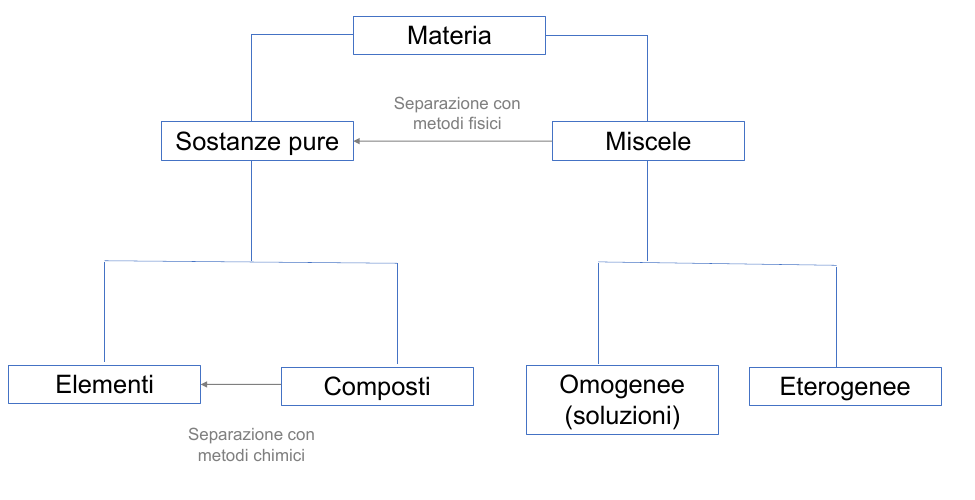
\includegraphics[width=\textwidth,height=\textheight,keepaspectratio]{immagini/grafico1}
	\label{fig:grafico1}
\end{figure}
\chapter{Teoria atomica}
\section{Teoria atomica di Dalton}
\begin{enumerate}
	\item Tutta la materia è costituita da atomi, piccole particelle indivisibili di un elemento che non possono essere nè create, nè distrutte
	\item Gli atomi di un elemento non possono essere convertiti in atomi di un altro elemento
	\item Gli atomi di un elemento sono identici nella massa e nelle altre proprietà e sono diversi dagli atomi di qualsiasi altro elemento \label{3}
	\item I composti sono formati dalla combinazione di uno specifico rapporto di atomi differenti
\end{enumerate}
\noindent La teoria di Dalton spiega le leggi delle combinazioni chimiche
\begin{itemize}
	\item Legge della composizione definita \hfil\\
	Indipendentemente dalla sua fonte, un particolare composto chimico è costituito dagli stessi elementi negli stessi rapporti in massa
	\item Legge della conservazione della massa \hfill\\
	In base al postulato \hyperref[3]{3} della legge di Dalton gli atomi, e quindi la loro massa, vengono conservati nelle reazioni chimiche
\end{itemize}
\section*{Scoperta delle particelle sub-atomiche: raggi catodici}
\begin{itemize}
	\item Il raggio devia in presenza di un campo elettrico o magnetico $\Rightarrow$ Consiste in particelle cariche di cui si determina il rapporto carica/massa
	\item In presenza di un campo elettrico esterno il raggio devia verso la rica positiva $\Rightarrow$ Consiste in particelle negative
	\item Il raggio è identico per ogni catodo $\Rightarrow$ Le particelle fanno parte di tutta la materia
\end{itemize}
\subsection*{Esperimento di Millikan}
\begin{figure}[H]
	\centering
	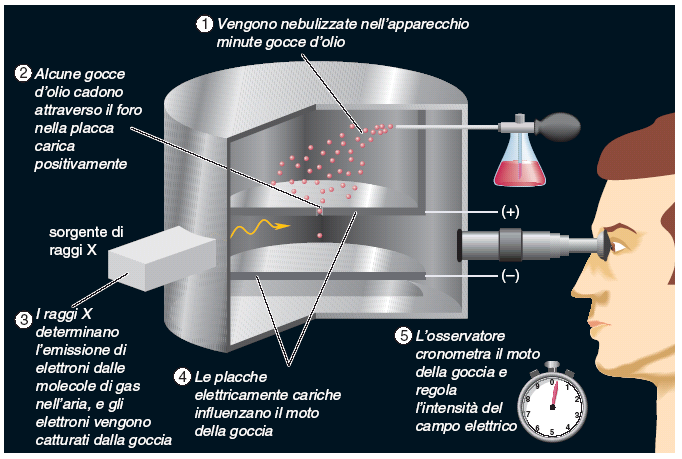
\includegraphics[width=0.5\textwidth,height=\textheight,keepaspectratio]{immagini/Millikan}
	\label{fig:millikan}
\end{figure}
\[\text{massa elettrone} = \left(\frac{massa}{carica}\right)carica = 9.109 \times 10^{-28}g  \]
\begin{figure}[H]
	\centering
	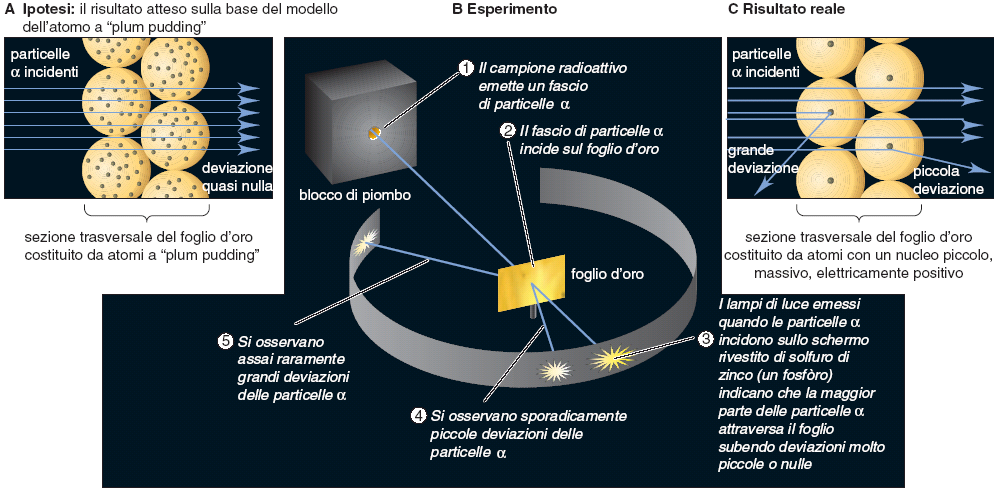
\includegraphics[width=\textwidth,height=\textheight,keepaspectratio]{immagini/atomo}
	\caption{}
	\label{fig:atomo}
\end{figure}
\begin{figure}[H]
	\centering
	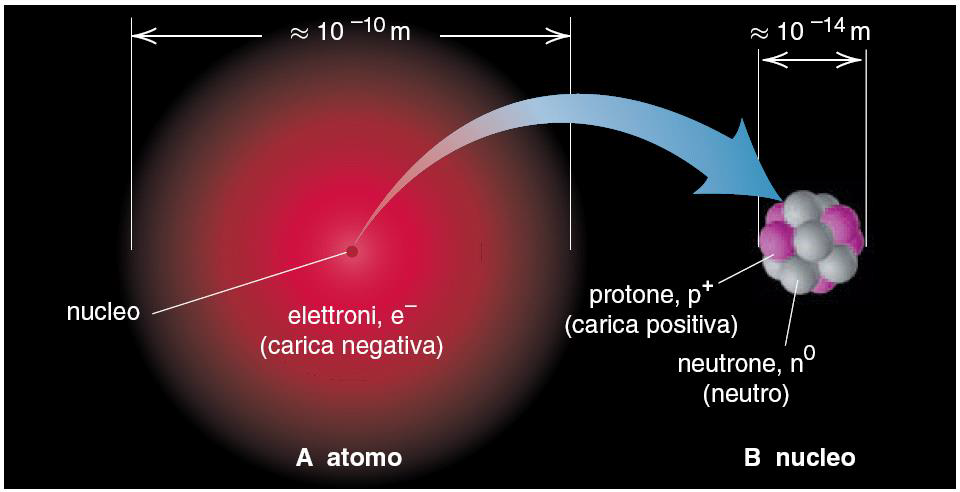
\includegraphics[width=0.5\linewidth, height=\textheight,keepaspectratio]{immagini/atomo1}
	\label{fig:atomo1}
\end{figure}
\begin{itemize}
	\item [A.] Una nuvola di elettroni carichi negativamente, in modo rapido, occupa pressochè tutto il volume atomico e circonda il minuscolo nucleo centrale
	\item [B.] Il nucleo contiene pressochè tutta la massa dell'atomo ed è costituito da protoni carichi positivamente e neutroni elettricamente neutri
\end{itemize}

\section{Simbolo atomico, numero atomico e numero di massa}

\begin{figure}[H]
	\centering
	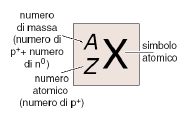
\includegraphics[width=0.2\linewidth, height=\textheight,keepaspectratio]{immagini/numero.png}
	\label{fig:numero}
\end{figure}

\begin{center}
\begin{tabular}{|c|c|}
	\hline
	X & simbolo atomico dell'elemento \\
	\hline
	Z & numero atomico (numero di protoni nel nucleo) \\
	\hline
	A & numero di massa	\\
	\hline
\end{tabular}
\end{center}

\[A = Z+N\]

\subsection*{Isotopi}

Gli isotopi sono atomi di un elemento con lo stesso numero di protoni, ma con diverso numero di neutroni; gli isotopi hanno lo stesso numero atomico, ma diverso numero di massa

\subsection*{Teoria atomica moderna}

\begin{enumerate}
	\item Tualla la materia è costituita da atomi. L'atomo è la particella più piccola che identifica univocamente un elemento 
 \item Gli atomi di un elemento non possono trasformarsi negli atomi di un altro elemento in una trasformazione chimica. Elementi possono convertiti in atri elementi solo in una reazione nucleare 
 \item Tutti gli atomi di un elemento hanno lo stesso numero di protoni e elettroni che determina il comportamento chimico dell'elemento. Gli isotopi di un elemento differiscono nel numero di neutroni, dunque nel numero di massa. Un campione di elemento viene considerato come se tutti i suoi atomi avessero una massa mediante
 \item i composti sono formati dalla combinazione chimica di due o più elementi in rapporti specifici
\end{enumerate}

\subsection*{Tecniche di separazione fondamentali}

\begin{description}
	\item[Filtrazione:] separa i componenti di una miscela sulla base di differenze tra le dimensioni delle particelle. La filtrazione viene usata spesso per separare un solido da un liquido 
 \item[Cristallizzazione:] la separazione è basata sulle differenze di solubilità dei componenti di una miscela 
 \item[Distillazione:] separa i componenti sulla base di differenze di volubilità 
 \item[Estrazione:] la separazione è basata sulle differenze di solubilità in diversi solventi
 \item[Cromatografia:] la separazione è basata sulle differenze di solubilità in una fase stazionaria     
\end{description}

\section{Atomi e molecole}
Una molecola è un'unità strutturale indipendente costituita da uno o più atomi, tenuto insieme da legami chimici (legami covalenti). Una molecola è la più piccola particella di una sostanza che ne mantenga la composizione e le proprietà chimiche. Le molecole sono le unità fondamnetali dei composti molecolari

\subsection*{Formule chimiche}
In una formula chimica, i simboli degli elementi e i pedici numerici indicano la specie e il numero di ciascun atomo presente nella più piccola unità della sostanza. Esistono più tipi di formule chimiche di una composto

\begin{description}
	\item[Formula empirica:] mostra il numero relativo di atomi in ciascun elemento nel composto. \'E il tipo più semplice di formula chimica
 \item[Formula molecolare:] mostra il numero reale di atomi di ciascun elemento in una molecola di composto
 \item[Formula di struttura:] mostra il numero di atomi e i legami tra di essi, cioè le posizioni reciproche e le connessione degli atomi nella molecola    
\end{description}

\begin{description}
	\item[Ione:] un singolo atomo (ione monoatomico) o un gruppo di atomi (ione poliatomico) legati mediante legami covalenti che ha una carica netta 
 \item[Catione:] ione di carica positiva (\# protoni > \# elettroni)
 \item[Anione:] ione di carica negativa (\# elettroni > \# protoni)  
\end{description}

\noindent I composti ionici sono costituiti da ioni, che sono l'unità fondamentale

\section{Stechiometri}
\subsection*{Studio delle relazioni di massa in chimica}

Masse atomiche: le masse relative gli atomi dei diversi elementi si esprimono secondo le loro masse atomiche 
\[u = \frac{1}{12}m(\ch{^{12}C})\]
Nella tavola periodica è riportata la massa atomica media pesata per l'abbondanza isotopica \newline
Massa molecolare: la massa molecolare si ottiene sommando le masse atomiche secondo la formula chimica \newline
Per i composti ionici si parla di massa forumla perchè i composti ionici non sono costituiti da molecole 

\subsection*{Mole}
Le trasformazioni chimiche avvengono in seguito a reazioni tra atomi, molecole o ioni; è quindi fondamentale conoscere il numero di atomi presenti nella massa di sostanza sottoposta a reazione. \newline
La \textbf{mole} (mol) è la quantità di sostanza che contiene tante entità elementari quante sono gli atomi in 12g di \ch{^{12}C}; il termine entità si riferisce ad atomi, ioni, molecole, unità di formula, elettroni - ogni tipo di particelle \newline
Una mole contiene $6.022\times 10^{23}$ entità; si chiama numero di Avogadro e si indica con $N_A$

\subsection*{Massa molare}
La massa molare M di una sostanza è numericamente uguale alla massa di una mole di sue entità espressa in grammi; per gli elementi monoatomici, la massa molare, espressa in grammi per mole, è numericamente uguale alla massa atomica, espressa in unità di massa atomica. La massa atomica si legge sulla tavola periodica \newline
Per gli elementi molari e per i composti, è necessario conoscere la formula per determinare la massa molare 
\noindent m: massa(g) \quad n: numero di moli (mol) \quad M: massa molare $\left(\frac{g}{mol}\right)$ \quad $N_A$: numero di Avogadro \newline 
N: numero di entità

\begin{align*}
	n = \frac{m}{M} \qquad  m &= nM \\
	n = \frac{N}{N_A} \qquad  N &= nN_A
\end{align*}

\noindent Per un elemento \qquad  Massa elemento $\xrightarrow[]{M}$ Quantità di massa $\xrightarrow[]{\text{numero di Avogadro}}$ atomi elementi \newline
Per un composto \qquad Massa composto $\xrightarrow[]{M}$ Quantità di composto $\xrightarrow[]{\text{numero di Avogadro}}$ Molecole di composto 

\subsection*{Percentuale in massa della formula chimica}
\[\% A = \frac{m_A}{m_{totale}} \times 100\]
La percentuale in massa può anche essere utilizzata per calcolare la massa di un particolare elemento in una data massa di composto

\subsection*{Formule empiriche}
La formula empirica è la formula più semplice di un composto che sia in accordo con le analisi elementari. Mostra i numeri di moli interi più piccoli e dà il numero di atomi relatico di ogni elemento

\subsection*{Formula molecolare}
La formula molecolare mostra il numero reale di atomi di ciascun elemento in una molecola di composto \newline
La formula molecolare è un multiplo secondo un numero intero della formula empirica 

\section{Equazioni chimiche}
Un'equazione chimica è un enunciato in formula che esprime le identitò e quantità delle sostanze che partecipano a una trassformazione chimica o fisica \newline

Una freccia indica la trasformazione dei reagenti nei prodotti; i reagenti si scrivono a sinistra, mentre i prodotti a destra \newline
L'equazione deve essere bilanciata: lo stesso numero e tipo di atomi deve comparire nei due membri dell'equazione 

\subsection*{Bilanciare un'equazione chimica}
\begin{itemize}
	\item traduzione dell'enunciato
 \item bilanciare gli atomi usando i coefficienti stechiometrici: le formule non possono essere modificate
 \item correggere i coefficienti se necessario
 \item verificare che l'equazione sia bilanciata
 \item specificare lo stato fisico
\end{itemize}

\subsection*{Calcoli stechiometrici}
I coefficienti in un'equazione chimica bilanciata rappresentano i numeri relativi di particelle di reagenti e prodotti e i relativi numeri di moli. Poichè le moli sono correlate alla massa, l'equazione può essere utilizzata per calcolare masse di reagenti e/o prodotti coinvolti in una data reazione; i rapporti molari derivanti dall'equazione bilanciata rappresentano i fattori di conversione 

\subsection*{Reazioni in sequenza}
Le reazioni avvengono spesso in sequenza: il prodotto di una reazione diventa il reagente della successiva; la reazione complessiva è la somma delle varie reazioni. Ogni sostanza che si forma in una reazione ed è utilizzata in quella successiva può essere eliminata

\subsection*{Reagenti limitanti}
Un reagente può limitare la quantità di prodotto che si formare. Il reagente limitante sarà completamente consumato nella reazione, mentre parte del reagente che non è limitante (eccesso) rimarrà inalterata alla fine della reazione 

\subsection*{Resa}
\begin{description}
	\item[Resa teorica:] quantità di prodotto calcolata utilizzando i rapporti molari dell'equazione bilanciata 
 \item[Resa effettiva:] quantitò di prodotto ottenuta nella realtà
\end{description}

\[\text{Resa percentuale } = \frac{\text{resa effettiva}}{\text{resa teorica}} \times 100 \]

\section{Percentuale in massa dalla formula chimica}
\begin{equation*}
	\% A = \frac{m_A}{m_{tot}} \times 100
\end{equation*}
La percentuale in massa può anche essere utilizzata per calcolare la massa di un particolare elemento in una data massa di composto

\section{Formule empiriche e molecolari}
La formula empirica è la formula più semplice di un composto che sia in accordo con le analisi elementari. Mostra i numeri di moli interi più piccoli e dà il numero di atomi relativo di ogni elemento 

\begin{es}
	La formula empirica del perossido di idrogeno è HO
\end{es}

\noindent La formula molecolare mostra il numero reale di atomi di ciascun elemento in una molecola di composto

\begin{es}
	La formula molecolare del perossido di idrogeno è $H_2O_2$
\end{es}

\subsection*{Determinare la formula molecolare}
La formula molecolare mostra il numero reale di atomi di ciascun elemento in 1 mole di composto. La formula molecolare è un multiplo intero della formula empirica
\begin{equation*}
	\frac{\text{massa molecolare (g/mol)}}{\text{massa della formula empirica (g/mol)}} = \text{multiplo intero}
\end{equation*}
Si possono avere diversi composti che hanno la stessa formula molecolare, ma con proprietà
\begin{es}
	Etanolo e Dimetiletere
\end{es}

\section{Equazioni chimiche}
Un'equazione chimica è un enunciato in formule che esprime le identità e le quantità delle sostanze che partecipano a una trasformazione chimica o fisica

\begin{es}
	\begin{equation*}
		H_2(g) + F_2(g) \longrightarrow 2HF(g)
	\end{equation*}
\end{es}

\noindent Una freccia indica la trasformazione dei reagenti nei prodotti; i reagenti si scrivono a sinistra, i prodotti si scrivono a destra \newline
L'equazione deve essere bilanciata: lo stesso numero e tipo di atomi deve comparire nei due membri dell'equazione \newline
Per bilanciare un'equazione chimica bisogna seguire i seguenti passaggi
\begin{enumerate}
	\item traduzione dell'enunciato
	\item bilanciare gli atomi usando i coefficienti stechiometrici: le formule non possono essere modificate
	\item correggere i coefficienti se necessario
	\item vericare che l'equazione sia bilanciata
	\item specificare lo stato fisico: solido (s), liquido puro (l), sostanza gassosa (g), ione o molecola in soluzione acquosa (aq)
\end{enumerate}
I coefficienti in un'equazione chimica bilanciata rappresentano i numeri relativi di particelle di reagenti e prodotti e i relativi numeri di moli; poicheè le moli sono correlata alla massa, l'equazione può essere utilizzata per calcolare masse di reagenti e/o prodotti coinvolti in una data reazione. I rapporti molari derivanti dall'equazione bilanciata rappresentano i fattori di conversione

\subsection*{Reazioni in sequenza}
Le reazioni avvengono spesso in sequenza: il prodotto di una reazione diventa il reagente della successiva. la reazione complessiva (reazione netta) è la somma delle varie reazioni. Ogni sostanza che si forma in una reazione ed è utilizzata in quella successiva può essere eliminata

\end{document}